\documentclass[final,5p,times,twocolumn,authoryear]{elsarticle}

\usepackage{amsmath}
\usepackage{amsfonts}
\usepackage{amssymb}
\usepackage{listings}
\usepackage{algorithm}
\usepackage{algorithmicx}
\usepackage{algpseudocode}
\usepackage{subfig}

\algnewcommand\algorithmicinput{\textbf{INPUT:}}
\algnewcommand\INPUT{\item[\algorithmicinput]}

\algnewcommand\algorithmicreturns{\textbf{RETURNS:}}
\algnewcommand\RETURNS{\item[\algorithmicreturns]}

\algnewcommand\algorithmicvars{\textbf{VARIABLES:}}
\algnewcommand\VARIABLES{\item[\algorithmicvars]}

\algnewcommand\algorithmicconsts{\textbf{CONSTANTS:}}
\algnewcommand\CONSTANTS{\item[\algorithmicconsts]}

\newcommand{\var}[1]{\mathit{#1}}
\newcommand{\func}[1]{\mathrm{#1}}

\DeclareMathOperator*{\argmax}{\arg\!\max}

\def\bibsection{\section*{References}}

\begin{document}
\begin{frontmatter}

\title{Decision-theoretic file carving}

\author[add1]{Pavel Gladyshev}
\ead{pavel.gladyshev@ucd.ie}
\author[add2]{Joshua Isaac James}
\address[add1]{Digital Forensics Investigation Research Laboratory, University College Dublin, Belfield, Dublin 4, Ireland}
\address[add2]{Digital Forensics Investigation Research Laboratory, Hallym University, 1 Hallimdaehak-gil, Chuncheon-si, Gangwon-do, South Korea}
\begin{abstract}
This article explores a novel approach to file carving by viewing it as a decision problem. It allows us to design algorithms that produce best effort results under the given resource constraints. It is important for digital forensic triage as well as for e-discovery. As an illustration, we develop a novel file carving algorithm together with a novel linear-time detector of JPEG data and examine its performance.
\end{abstract}

\begin{keyword}
decision-theoretic file carving \sep 
file carving \sep 
digital forensic investigation \sep 
Digital forensic triage \sep
preliminary analysis
\end{keyword}
\end{frontmatter}

\section{Introduction}

Digital forensic investigations must process large amounts of evidential data with limited resources \citep{Casey2009, pollitt2013triage}. Modern solutions to the data processing problem combine advances in automatic detection of relevant data with some form of selective human exploration to identify sample data and to validate output results \citep{marturana2013machine, schell2007cyber, james2014measuring}. Despite significant time and cost savings that automation can bring to digital investigations, this approach still relies on exhaustive processing of the suspect data.

Various methods have been proposed that attempt to prioritise exhibits by first prioritising suspect data sources that the exhibit contains \citep{shaw2013practical, rogers2003role, overill2013triage}. Several works \citep{Koopmans2013,Casey2009} have discussed the idea of digital forensic triage; an investigation processes with the goal of not always requiring an exhaustive search of all devices, -and helps with decisions of relevancy and prioritisation.

There are many situations where a digital investigator is limited either in time or available computational power. For example, a parole officer may use a portable forensic tool to periodically check that an offender's computer does not contain child abuse material. The time and processing power available to the officer on site is limited and -- given the growth in data storage capacity -- may not be sufficient to exhaustively explore the contents of an offender's computer. Thus a solution is required that would combine automatic processing with probabilistic sampling and prioritisation aimed at discovering relevant information more quickly.

This paper explores the idea of probabilistic sampling and prioritisation in the context of file carving. It shows that when the investigator is looking for files of a particular kind, such as large JPEG files, this information can be used to speed up file carving by prioritizing processing of data blocks that are most likely to contain relevant data. This is demonstrated by constructing specialised file carver for digital photographs that outperforms\footnote{The relevant measure of performance is discussed in Section \ref{utility-of-carving}} traditional file carvers.

\subsection{Contribution}
This work contributes to the field of digital forensic investigation by proposing a \emph{best-effort} file carving method that aims to recover as much relevant information as possible under the given time- and processing power constraints. It is suitable for digital forensic triage purposes as defined by \citep{Koopmans2013}. Specifically, this work provides:
\begin{itemize}
	\item{a formal statement of file carving as decision problem;}
	\item{an illustration of how simplifies mathematical models and simulation can help improving file carving efficiency;}
	\item{a JPEG image carving algorithm and software application that could recover potentially relevant images (photographs) faster than traditional carvers.}
\end{itemize}

\section{Sequential file carving}

File carving is often used in digital investigations. Traditional file carving programs, like {\tt foremost} by \citep{richard2005scalpel} or {\tt photorec} by \citep{grenier2007photorec} can be described as \emph{sequential} file carvers. The basic sequential carving algorithm works as follows: the carving starts at the first data block of the drive and progresses consecutively until the end of the drive is reached. Each block is checked against a database of header and footer signatures. If the block matches some \emph{header} signature, it is assumed to be the first block of a file to be recovered. The rest of the file is assumed to occupy the subsequent consecutive blocks up to and including the matching ``footer'' block. If the ``footer'' block cannot be found, the length of the recovered file is capped at a predefined limit. 

Sequential file carving works because the mainstream file systems are designed to store file data in consecutive disk blocks whenever possible, in order to maximize performance of mechanical hard disk drives. While file fragmentation does occur, \citep{garfinkel2007carving} shows that the majority of files in personal computers are not fragmented.  

Prior research in file carving mainly focused on improving accuracy; more accurate techniques for detecting file fragments of particular kinds were proposed\footnote{For more detail see \citep{Veenman2007statistical}, \citep{li2011novel}, and \citep{Garfinkel2015hashbased}}, and algorithms for detection and reassembly of fragmented files were developed that achieve quadratic time complexity\footnote{$O(n^2)$ time complexity where $n$ is the number of fragments to be reassembled. For more detail see \citep{memon2006automated}}. 

The performance of the basic sequential carving algorithm was improved upon by Richard, et al \citep{Richard2007inplace}, and similarly Meijer \citep{MeijerRob2012}, who proposed in-place\footnote{Also known as zero-storage} file carving in an attempt to lower the time and space requirements compared to traditional sequential carving. These approaches identify the challenges with traditional file carving, and propose methods to reduce carving resource requirements by minimizing the amount of disk I/O associated with copying recovered file data. Essentially, once file data is discovered, pointers are created in virtual file systems that point to the data directly on the suspect disk rather than copying data from the suspect disk. However, the approach used for \emph{finding} the file data is still sequential, as before.

\section{File carving as a Battleships game}

File carving is a process of exploration, and it is instructive to consider file carving as an analogy of the Battleships\footnote{The Battleships game is played as follows: each player has a pad of paper with two 100-square grids (maps) -- one for arranging the player's ships and the other for noting the discovered locations of the opponent's ships. Before the start of the game, each player secretly arranges their ships on their grid. A ship occupies a number of consecutive squares and is oriented either vertically or horizontally. The ships cannot overlap. The game proceeds in turns with each player sending a "bomb" to a particular square on the enemy grid. The other player then responds whether the "bombing" succeeded in damaging one of their ships. A ship is destroyed when all of the squares it occupies are hit by the opponent. The game ends when one of the players completely destroys the other player's fleet.} game, in which one player -- the data storage -- arranges her ships (the relevant files) on a ``canal'' and the other player -- the file carver -- tries to destroy the opponent's ships with the minimal number of bombs (see Fig. \ref{fig:battleships_on_a_canal}).  

The simplest strategy that is guaranteed to destroy the opponent's fleet is to bomb all squares consecutively from left to right, which is precisely what sequential carvers do. Although effective, this strategy is not necessarily the most efficient. A human players of Battleships would randomly bomb the opponent's map until one of the ships is hit. After that, she would bomb the adjacent squares until the damaged ship is completely destroyed. It is intuitively plausible that similar approach could be used in file carving and that it may outperform sequential carving algorithms. In the rest of this paper we present theoretical and experimental results that validate this intuition using ecision theory, numeric simulation, and actual file carving experiments.

\begin{figure*}
  \centerline{\includegraphics[width=0.6\textwidth]{fig3}}
  \caption{A 1-dimensional Battleships game.}
  \label{fig:battleships_on_a_canal}
\end{figure*}

\subsection{Decision theory basics}

Decision theory is a branch of mathematics that studies decision making. In its basic form, it represents decision as a choice between several alternative actions that together form the set $A$ (possible actions): 

\begin{equation}
A=\left\{a_1,a_2,\dots,a_n\right\}
\end{equation}

Any chosen action $a_i \in A$ can result in one of several possible, mutually exclusive outcomes that together form the set $O$ (possible outcomes):  

\begin{equation}
O=\left\{o_1,o_2,\dots o_m \right\}
\end{equation}

The likelihood of a particular outcome $o_j \in O$ happening as a result of the action $a_i \in A$ is represented by the conditional probability $P(o_i \mid a_i)$. 

The desirability of a particular outcome is modelled by the \emph{utility} function $u()$ that assigns a real-valued score to each outcome. The higher the utility score, the more desirable is the outcome. The cost associated with doing a particular action can be modeled as a reduction of utility scores of the corresponding outcomes. To model it formally we define $u()$ as function of both the outcome \emph{and} the action:

\begin{equation}
u : O \times A \rightarrow \mathbb{R}
\end{equation} 

The principle of \emph{Maximum Expected Utility} (MEU) states that a rational decision maker should choose the action with the highest mathematical expectation of the utility score across all possible outcomes:

\begin{equation} \label{eq:decision}
a = \argmax_{a_i \in A}\sum_{o_j \in O} u(o_j,a_i)P(o_j \mid a_i )
\end{equation}

\subsection{File carving as decision problem}

Like a player of Battleships that chooses which square to bomb, file carver chooses which disk block to process next. Let array $B$ represent the drive subjected to file carving:

\begin{equation}
B=\left(b_0,b_1,\dots b_m \right)
\end{equation}

Each element $b_0 \dots b_m$ represents a separate data block on the drive. 

Let file carving \emph{action} be the act of processing a particular disk block $b_k \in B$. There are two possible outcomes: $b_k$ contains the relevant data ($r$), or $b_k$ does not contain relevant data ($n$):

\begin{equation}
O=\left\{r,n\right\}
\end{equation}

Given that hard disk drives have physical read-write heads, that may have to be repositioned to access a different disk block, it is convenient to \emph{refer} to a particular block by its \emph{offset} from the last processed block. We will use such offsets instead of block indices to identify actions that can be taken by the carver:

\begin{equation}
A=\left\{\dots,-3,-2,-1,1,2,3\dots\right\}
\end{equation}

For example, if the last processed block was $b_{10}$, the action $a=-3$ means examination of the block $b_7$. 

\subsubsection{Utility of file carving actions}
\label{utility-of-carving}

In triage situations it is important to get relevant files quickly. Sequential carving takes long time to find relevant files if they are spread throughout the disk space. Figure \ref{fig:sequential} shows a plot of the total amount of data recovered by a sequential carver as function of time. Steep climbs occur when the carver finds relevant data; long horisontal stretches occur when the carver scans through drive areas devoid of relevant data. Figure \ref{fig:sequential} clearly shows that utility of carving actions can be defined as the \emph{slope} of that curve:

\begin{equation}
\label{eqn:utility-def}
u(o,a)=\begin{cases} 
      0 & o = n \\
      \frac{1}{T_{proc}(a)} & o = r 
   \end{cases}
\end{equation}
where
\begin{equation}
T_{proc}(a) = t_{RAM} + t_{seek}(a)
\end{equation}

Definition (\ref{eqn:utility-def}) consists of two parts. The first part of it says that processing blocks containing irrelevant data has zero utility in the sense that it does not increase the total amount of recovered data. The second part states that the usefulness of processing a block of relevant data is determined by how fast we process it -- the slower we process it, the more gentle is the slope of the curve in Figure \ref{fig:sequential}, and lower the utility of it. 

$T_{proc}(a)$ is the time required to process a disk block. It consists of a relatively constant component $t_{RAM}$ -- the time required to read a block of data into RAM and process it there, and $t_{seek}(a)$ -- the drive seek time\footnote{the time taken for a disk drive to locate the area on the disk where the data to be read is stored.} that generally depends on how far the target data block is from the last processed block. If the block at the offset $a$ contains relevant data, its utility is the reciprocal of $T_{proc}(a)$.

\begin{figure*}
	\center
	\includegraphics[width=0.9\textwidth]{wc_fig}
	\caption{The total amount of data recovered by a sequential file carver as a function of time. In this example the relevant data (JPEG images) occupied approximately 5\% of a 32Gb disk image.}
	\label{fig:sequential}
\end{figure*}

The substitution of  (\ref{eqn:utility-def}) for $u(o,a)$ in (\ref{eq:decision}) produces the deicsion principle for file carving:

\begin{equation} \label{eq:carving-decision}
a = \argmax_{a \in A} \left( \frac{1}{T_{proc}(a)} p(a,l)\right)
\end{equation}

where function $p(a,l) = P(o=r \mid a,b_l)$ represents the probability of finding a relevant data block at a particular offset $a$ from the last processed block $b_l$. Parameter $l$ is the index of the last processed block: $0 \leq l \leq m$. Function $p(a,l)$ represents the current ``knowledge'' of the carver of where the relevant blocks are likely to be and serves as a scaling factor reducing the benefit of processing a particular block if that block is unlikely to contain relevant data.

To implement a carver based on the Equation (\ref{eq:carving-decision}), the following things are required:

\begin{enumerate}
\item{a reliable and efficient method to detect \emph{relevant} data blocks. Unlike the header and footer signatures used in sequential carving, this method should work for arbitrary blocks from the middle of the file;}
\item{an understanding of the shape and properties of $p(a)$ in the context of a particular carving task, and how $p(a)$ changes when some block is examined and found to be either relevant or irrelevant;}
\item{an efficient way to determine $\argmax_{a \in A} \left( \frac{1}{T_{proc}(a)} p(a,l)\right)$ at run time.}

\end{enumerate}

It is also important to understand and practically demonstrate the circumstances in which decision-theoretic file carver would outperform sequential file carver. To prove the viability of decision-theoretic carving we developed a specialised file carver for recovering large JPEG files. 

\section{The need for selective recovery of large JPEG files}

Suppose that parole officer needs to check the computer of a sex offender for presence of raw digital photographs that may indicate production of child abuse material. To do it, she or he needs a program that can quickly find as many raw digital photographs as possible. The computer in question may not have much processing power, and the time for analysis may be limited. Decision-theoretic approach fits this problem very well, because it focuses on making best decision at every step leading to the best-effort results under given circumstances.  

A digital camera sensor typically produces raw photographs at a fixed resolution. The raw sensor data is then resized and compressed according to the image quality settings specified by the user. The resulting JPEG file is, typically, several megabytes in size. 

Figure \ref{fig:jpeg-dist} shows a histogram of sizes of digital photographs from a personal collection of 5000 digital photographs accumulated over 10 years. There are several peaks corresponding to different cameras and image quality settings used over the years. Each peak resembles the ``bell curve'' of the normal distribution\footnote{Recall that JPEG encoding divides the image into square fragments $8 \times 8$ pixels. Every such fragment is compressed independently meaning that by the central limit theorem of probability theory, the probability distribution of JPEG sizes for a particular camera setting converges to normal (Gaussian) distribution.}. Note that the vast majority of JPEG files in Figure \ref{fig:jpeg-dist} are bigger than 700 Kb in size. The two right-most peaks in the histogram correspond to images produced by a newer camera, whose JPEG files a bigger than 2000 Kb. It is highly likely that mainstream camera resolution will continue to grow leading to larger size of JPEG files. 

\begin{figure*}
  \centerline{\includegraphics[width=0.9\textwidth]{jpeg-sizes}}
  \caption{Histogram of actual file sizes from a personal collection of raw digital photographs in JPEG format. Horizontal axis is the size of files in Kibibytes, vertical axis is the number of files. Each of the peaks visible in the histogram corresponds to a particular camera and image size and quality settings.}
  \label{fig:jpeg-dist}
\end{figure*}

\section{Detector of JPEG data}
\label{sec:detector}

A fast and accurate detector of relevant data is essential for efficient operation of decision-theoretic file carver. Our initial implementation of JPEG data detector used Support Vector Machine (SVM) classifier based on the ideas of Li \emph{et al.} described in \citep{li2011novel}. The detector used 256 data features corresponding to byte-value frequencies. The detector was trained using 17,918 training samples that contained 8,985 samples from known Non-JPEG files and 8,933 samples from known JPEG files. It included samples from all sections of JPEG files. After training the detector was tested on a much larger data sample derived from a different source. It demonstrated 99\% true positive rate and 33\% false positive rate. 

The high false positive rate is due to relatively high entropy of compressed JPEG data. According to our tests the trained linear SVM classifier did not distinguish JPEG data from other high-entropy data, such as ZIP files. As we shall see in Section \ref{sec:implement}, the high false positive rate of the detector can make decision-theoretic carving highly inefficient. In a nutshell, SVM-based detector forced our carver to spend a lot of time looking for JPEGs in non-JPEG high-entropy files (ZIP, GIF, RAR files, etc.). As a result, our carver behaved more like a typical sequential carver. The development of efficient and accurate detector of relevant data is, therefore, essential problem in decision-theoretic carving. 

Clearly, an accurate detector of relevant data can be constructed only if the target data has features that reliably distinguishes it from any other data. Even if such features are present, it may not be possible to compute them efficiently\footnote{Consider, for example, the problem of selectively carving child pornography images from unallocated disk space}. Since the aim of this paper was to \emph{demonstrate} viability of the decision-theoretic carving, we developed a simple \emph{ad-hoc} detector for JPEG data that provided acceptable precision and performance characteristics for our experiments (Algorithm \ref{alg:detector}).  

Our detector relies on the presence of escape sequences in JPEG data. Escape sequences are used by JPEG encoder for in-band signalling. When a byte value of 255 is encountered in the JPEG stream, JPEG decoder treats is as the beginning of a command. The subsequent bytes specify what the JPEG decoder must do. For disambiguation purposes any actual 255 data value is encoded as 255 followed by 0.  Our detector defines JPEG data as any high entropy data that contains at least one JPEG escape sequence. Instead of calculating the actual entropy measure, it constructs a histogram of byte values from the given data block and checks that no single value occurs exceedingly often.

\begin{algorithm}[ht]
\begin{algorithmic}
    \\
    \INPUT 
    \\ {array $d[N]$ of $N$ eight-bit bytes.}
    \RETURNS 
    \\ {\underline{true} if $d$ contains JPEG data, \underline{false} otherwise.}
    \VARIABLES 
    \\ {integer array $c[256]$ for counting distinct byte values in $d$, \\ integer variable $esc$ for counting JPEG escape sequences.}
    \\
    \State $esc \gets 0$\Comment{Initialize counters}
    \For{$i=0$ \textbf{to} $255$}
       \State $c[i] \gets 0$
    \EndFor
    \\
    \For{$i=0$ \textbf{to} $N-2$} \Comment{Iterate over $d$}
       \State $val \gets d[i]$
       \State $nextval \gets d[i+1]$
       \\
       \State $c[val] \gets c[val]+1$ 
       \\
       \If{$c[val] > 50$}  

          \Return \underline{false} \Comment{all values should be equally infrequent}
       \EndIf
       \\
       \If{$val = 255$ and $nextval = 255 $}

          \Return \underline{false} \Comment{A 255 must not be followed by 255}
       \EndIf
       \\
       \If{$val = 255$ and $nextval \in \{0,208,209,\dots,215\} $}

          \State $esc \gets esc+1$ 
       \EndIf       
    \EndFor 
    \\
    \If{$esc > 0$}
    
		\Return \underline{true} \Comment{Must contain at least one escape seq.}
    \Else
    
        \Return \underline{false}
    \EndIf       
    
\end{algorithmic}
\caption{Simple detector of JPEG data ($JpegDetect$)}
\label{alg:detector}
\end{algorithm}

Observe that Algorithm \ref{alg:detector} is quite efficient. It has linear time complexity with respect to the size of $d$. This is similar to the complexity of signature-based detection methods used in mainstream file carvers.  

\section{Probability of finding JPEG data in a particular block on the drive}
\label{sec:probability}

The second problem that needs to be solved to create a decision-theoretic JPEG carver is to determine the probability of finding a piece of JPEG digital photograph in a particular data block on the suspect hard disk drive. For the purposes of this article we decided to build a simplified mathematical model of the JPEG carving problem and explore its properties using small-scale simulation. 

We make the following core assumptions about JPEG files:

\begin{enumerate}
\item{JPEG files are not fragmented;}
\item{JPEG files do not overlap and do not share blocks;}
\item{the only other information we have about the target files is the minimal and maximal file size limits specified in the file carver configuration settings.} 
\end{enumerate}

According to the principle of uninformed priors \citep{jaynes2003probability}, we ought make the following additional assumptions:

\begin{enumerate}
\setcounter{enumi}{4}
\item{JPEG file sizes are uniformly distributed between minimal and maximal limits;}
\item{starting locations of JPEG files are uniformly distributed throughout the disk space subject to non-fragmentation and non-overlapping requirements;}
\item{starting locations of JPEG files are uniformly distributed throughout the disk space subject to non-fragmentation and non-overlapping requirements;}
\item{the total number of blocks occupied by relevant data is not known and the probability that the relevant data occupies a certain amount of disk space is uniformly distributed between 0 and 100 percent.}
\end{enumerate}

\subsection{Estimating probability function with small-scale simulation}

To get a sense of the shape and properties of The probability of encountering JPEG  data in a particular block $P(o=r | b_i)$, we performed a series of small-scale simulations using a ``toy'' model of a hard disk drive with only 20 blocks: $B=(b_0,\dots,b_{19})$. The model represents each block with a single value: the value of 1.0 corresponds to blocks containing JPEG data while 0.0 represents blocks with irrelevant information. The small number of blocks in the model allowed brute-force computation of $P(o=r | b_i)$ by constructing all possible ``contents'' of the drive satisfying the assumptions about the location and sizes of JPEG files. The value of  $P(o=r | b_i)$ for a particular block $b_i$ is calculated as the frequency of $b_i$ containing JPEG data across all constructed disk contents\footnote{The corresponding python script \texttt{simulator.py} can be found in the source code of our carver \citep{gladyshevjames2015}.}.

We began our analysis by considering a very simple case: the drive contains single fixed-size JPEG file. The results of the small scale simulation are shown in Figure \ref{fig:fig-20blk-11min-11max2d}. The plot of $P(o=r|b_i)$ has trapezoidal shape. To see why it is so, consider Figure \ref{fig:pa_explan}. Under the assumption of non-fragmentation, an 11-block continuous JPEG file can reside in one of 10 possible positions on a 20-block drive. Observe that two blocks in the middle of the drive are occupied in every possible position of the file, while the very first and the very last blocks on the drive are occupied only in one of ten possible positions of the file. That results in a trapezoidal form of the probability distribution $P(o=r|b_i)$ seen in Figure \ref{fig:fig-20blk-11min-11max2d}.

\begin{figure*}
  \centerline{\includegraphics[width=0.9\textwidth]{fig-20blk-11min-11max2d}}
  \caption{Probability of finding relevant data in a particular disk block, assuming that JPEG files are \emph{exactly} 11 blocks in size.}
  \label{fig:fig-20blk-11min-11max2d}
\end{figure*}

\begin{figure*}
  \centerline{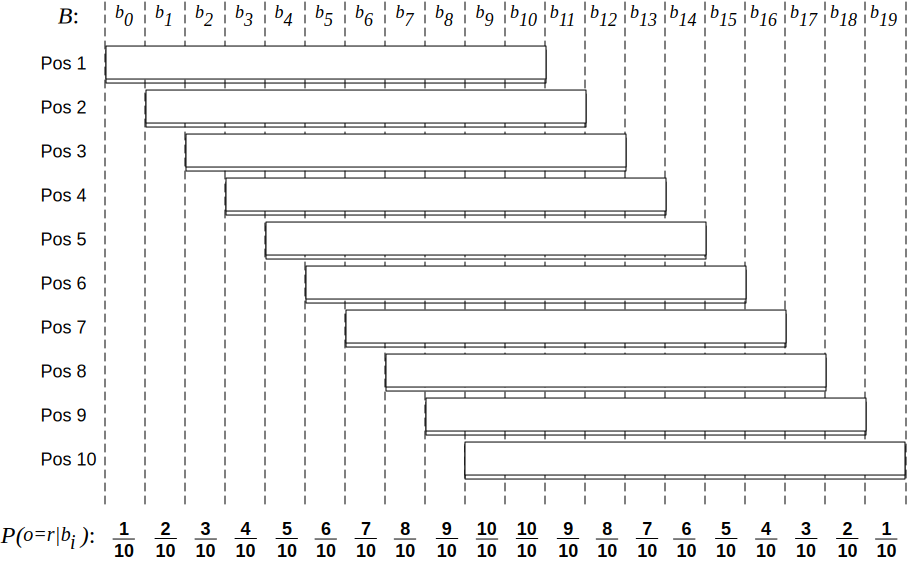
\includegraphics[width=\textwidth]{pa_explain.pdf}}
  \caption{Explanation of the trapezoidal form of the $p(a)$ probability distribution in Figure \ref{fig:fig-20blk-11min-11max2d}.}
  \label{fig:pa_explan}
\end{figure*}

Another case we considered is when the drive contains several non-fragmented files of the same size. Figure \ref{fig:fig-20blk-6min-6max3d} shows the results of the corresponding small scale simulation. In this example we reduced the fixed length of JPEG file down to 6 blocks, and our 20-block drive can now contain up to three such files. For the sake of clarity we added the third dimension to the plot: the total amount of JPEG data blocks stored on the drive. It allows us clearly see the probability $P(o=r|b_i)$ when the drive has either 1, 2 or 3 JPEG files stored on it. To better understand the shapes of these probability plots, the following flashlight analogy could be helpful: imagine an electric flashlight that takes three D-type batteries. A single battery can slide freely inside the flashlight. If we find a flashlight with a single battery inside laying on the floor, the exact position of the battery inside the case is somewhat uncertain to us, which corresponds to the first trapezoidal probability ``ridge'' in Figure \ref{fig:fig-20blk-6min-6max3d}. If, on the other hand, we know that all three batteries are in the flashlight, then we are quite certain where they are inside the flashlight. It corresponds to the last row of three probability ``ridges'' in \ref{fig:fig-20blk-6min-6max3d}, which are considerably higher than the first.

Note also, that if we see someone else's flashlight on the floor and have no prior information about the number of batteries in it, we ought to assume all possible battery configurations equally likely, and base our decision making on the probability plot that is the average of probability plots for all possible number of batteries inside.

\begin{figure*}
  \centerline{\includegraphics[width=0.9\textwidth]{fig-20blk-6min-6max3d}}
  \caption{Probability of finding relevant data in a particular disk block, given that certain number of blocks are occupied by relevant data and assuming that JPEG files are \emph{exactly} 6 blocks in size.}
  \label{fig:fig-20blk-6min-6max3d}
\end{figure*}

The final case we considered was the drive that contains a number of JPEG files above certain size. The corresponding simulation results are shown in Figure \ref{fig:fig-20blk-6min-20max3d} and Figure \ref{fig:fig-20blk-6min-20max2d}. The latter is the average probability plot assuming that all possible file configurations on the drive are equally likely. 

\begin{figure*}
  \centerline{\includegraphics[width=0.9\textwidth]{fig-20blk-6min-20max3d}}
  \caption{Probability of finding relevant data in a particular disk block, given that certain number of blocks are occupied by relevant data and assuming that JPEG files are \emph{at least} 6 blocks in size.}
  \label{fig:fig-20blk-6min-20max3d}
\end{figure*}

\begin{figure*}
  \centerline{\includegraphics[width=0.9\textwidth]{fig-20blk-6min-20max2d}}
  \caption{Probability of finding relevant data in a particular disk block, assuming that JPEG files are \emph{at least} 6 blocks in size.}
  \label{fig:fig-20blk-6min-20max2d}
\end{figure*}

A notable feature of the Figure \ref{fig:fig-20blk-6min-20max2d} is the presence of two peaks that make it look somewhat like a cat's head. Each of the peaks is located at the offset corresponding to the minimal file length away from each end of the drive. These peaks offer a slightly higher probability of finding JPEG data there, than on the rest of the drive, and -- if $\frac{1}{T_{proc}(a)}$ is constant -- these peaks are the optimal choices for the decision-theoretic block testing according to the Equation (\ref{eq:carving-decision}).

\subsection{Simulating results of successful and unsuccessful block testing}

Our model can also be used to explore the result of testing a particular block on the drive and finding either relevant or irrelevant data there. This is achieved by restricting probability calculation to only those drive configurations that either do or do not contain relevant data in the tested block. 

Figure \ref{fig:fig-20blk-6min-20max-testloc-5-0-2d} shows the result of testing the drive block $b_5$ corresponding to the first probability peak in Figure \ref{fig:fig-20blk-6min-20max2d} and finding no JPEG data there. Observe that the negative test at $b_5$ implies that blocks $b_0 \dots b_4$ also do not contain JPEG data. It is the consequence of assuming a lower bound of 6 blocks on JPEG file size together with the absence of fragmentation. 

\begin{figure*}
  \centerline{\includegraphics[width=0.9\textwidth]{fig-20blk-6min-20max-testloc-5-0-2d}}
  \caption{Posterior probability of finding JPEG data in a particular disk block, after testing $b_5$ and finding no relevant JPEG data there. All JPEG files are assumed to be at least 6 blocks in length.}
  \label{fig:fig-20blk-6min-20max-testloc-5-0-2d}
\end{figure*}

Note also that the shape of the posterior probability distribution to the right of $b_5$ is quite similar to the form of the initial probability distribution from Figure \ref{fig:fig-20blk-6min-20max2d}. The difference is that the first peak of probability is now at the block $b_{11}$ instead of $b_{5}$. This is again a direct consequence of the non-fragmentation assumption and the minimal file size assumption. 

The implication of the Figure \ref{fig:fig-20blk-6min-20max-testloc-5-0-2d} is that we may not always need to check every block on the drive to find all JPEGs above certain size. In the small-scale model from Figure \ref{fig:fig-20blk-6min-20max-testloc-5-0-2d} it suffices to check only three blocks: $b_5$,$b_{11}$, and $b_{14}$ to establish that there is no JPEGs on the 20-block drive! The larger the minimal size of JPEG files, the less blocks we need to check.

Figure \ref{fig:fig-20blk-6min-20max-testloc-5-1-2d} shows the result of testing drive block $b_5$ and finding that it contains relevant data. As expected, positive test increases the probability of finding JPEG data at $b_5$ to $1.0$. Note that the next most likely blocks to contain JPEG data are blocks $b_4$ and $b_6$ adjacent to $b_5$. This result is in full accordance with the human intuition of how to play the Battleships game: once an enemy ship is discovered by random bombing, human player finishes it by bombing squares adjacent to the first successful hit.

\begin{figure*}
  \centerline{\includegraphics[width=0.9\textwidth]{fig-20blk-6min-20max-testloc-5-1-2d}}
  \caption{Posterior probability of finding JPEG data in a particular disk block, after testing $b_5$ and finding that it contains JPEG data. All JPEG files are assumed to be at least 6 blocks in length.}
  \label{fig:fig-20blk-6min-20max-testloc-5-1-2d}
\end{figure*}

\section{Exploring properties of $T_{proc}(a)$ for hard disk drives and solid state drives.}
\label{sec:tproc}

The final piece of knowledge that needs to be acquired in order to build a decision-theoretic carver is the form and properties of $T_{proc}(a)$. In order to better understand its properties for actual HDD and SSD devices, we performed a series of experiments on a 120Gb Fujitsu HDD and a 120Gb SSDNow SSD. 

Two types of experiments were performed: one group of experiments measured $T_{proc}(a)$ for random block access, and the other group of experiments measured sequential access time. Given below is the summary of our findings.

To measure the time required for random block access, 1,000 random block tests were performed for each drive. Each random block test consists of a drive seek operation followed by reading the target disk block and performing JPEG data detection on the read data using Algorithm \ref{alg:detector}. The time required to complete each experiment was measured. We denote this time as $T_{rbt}(a)$. Figures \ref{fig:seek_time_hdd} and \ref{fig:seek_time_ssd} show the empirical $T_{rbt}(a)$ values for the 120Gb HDD and 120Gb SSD respectively. 

\begin{figure*}
  \centerline{\includegraphics[width=0.9\textwidth]{seek-time-hdd}}
  \caption{Time of random block testing on Fujitsu 120 Gb HDD.}
  \label{fig:seek_time_hdd}
\end{figure*}

\begin{figure*}
  \centerline{\includegraphics[width=0.9\textwidth]{seek-time-ssd}}
  \caption{Time of random block testing on SSDNow 120 Gb SSD.}
  \label{fig:seek_time_ssd}
\end{figure*}

The experimental data is quite noisy, which is probably due to RAM caching of the previously read blocks and fluctuations of normal system activity. Nevertheless, it suggests linear relationship between the absolute seek distance $|a|$ and processing time:

\begin{equation} \label{eq:tproc-eq}
T_{rbt}(a)=\beta |a|+\gamma
\end{equation}

where $\beta$ and $\gamma$ can be estimated using linear regression of the experimental data. The resulting linear approximations are shown in Figures \ref{fig:seek_time_hdd} and \ref{fig:seek_time_ssd} as dashed lines. We observe that in both cases $T_{rbt}(a)$ has relatively large constant component($\gamma$) and very shallow slope ($\beta$). In SSD experiments $\beta$ is almost zero and $T_{rbt}(a)$ is essentially a constant over the entire range of seek offsets. In HDD experiments $T_{rbt}(a)$ clearly increases proportionally to the seek offset, but despite a pronounced visual appearance in Figure \ref{fig:seek_time_hdd}, the sloping angle of $T_{rbt}(a)$ is actually so shallow and that it can be ignored at short travel distances like the size of a large JPEG file (see footnote\footnote{According to the estimates shown in Figure \ref{fig:seek_time_hdd}, HDD seek time increases from around 15 ms for short jumps to approximately 32 ms for jumps across the entire 120 Gb of the HDD. Most JPEGs are under 50Mb in size. At such small distances the increase of $T_{rbt}(a)$ would be only 0.007 ms or 0.0005\% of the constant 15 ms. Thus, for short jumps comparable to the size of JPEG file, we can assume $T_{rbt}(a)$ to be constant.} for explanation).

Although random block access is important for decision-theoretic carving, we should not overlook properties of sequential block access on SSD and HDD. It is well known that both SSDs and HDDs are optimised for sequential block access, and it is much quicker to read 100 blocks sequentially rather than randomly. Suppose that our file carver needs to examine content of a block at a (positive) offset $a$ from the last examined block. This can be done either by a direct jump followed by the block processing or by reading and processing consecutive blocks up to and including the target block. To distinguish the two approaches we denote the time required to read and examine $a$ consecutive blocks sequentially as $T_{seq}(a)$.

To determine how these approaches compare, we conducted additional experiments measuring the time taken to read and apply signature matching to large stretches of consecutive blocks on the 120Gb Fujitsu HDD and the 120Gb SSDNow SSD. As expected, $T_{seq}(a)$ grows at a rate proportional to $a$ for both SSD and HDD. To compare the behaviour of $T_{rbt}(a)$ and $T_{seq}(a)$, we plotted them together for the SSD (Figure \ref{fig:processing_time_ssd}) and HDD (Figure \ref{fig:processing_time_hdd}) respectively. 

\begin{figure*}
  \centerline{\includegraphics[width=0.9\textwidth]{processing-time-ssd}}
  \caption{$T_{rbt}(a)$ and $T_{seq}(a)$ calculated for SSDNow 120 Gb SSD.}
  \label{fig:processing_time_ssd}
\end{figure*}

\begin{figure*}
  \centerline{\includegraphics[width=0.9\textwidth]{processing-time-hdd}}
  \caption{$T_{rbt}(a)$ and $T_{seq}(a)$ calculated for Fujitsu 120 Gb HDD.}
  \label{fig:processing_time_hdd}
\end{figure*}

It is easy to see that $T_{seq}(a)$ is smaller for small values of $a$, while $T_{rbt}(a)$ is smaller for large values of $a$. The point of equivalence is $e$ where

\begin{equation}
  T_{rbt}(e)=T_{seq}(e)
\end{equation}

It is hardware-dependent and in our experiments it varied between $10^2$ and $10^3$ 4Kb blocks for SSDs and between $10^4$ and $10^5$ 4Kb blocks for HDDs.

\section{Designing new carving strategy for large, non-fragmented JPEG files}
\label{sec:decision}

Based on the results of Sections \ref{sec:detector}, \ref{sec:probability} and \ref{sec:tproc} we are now in a position to propose a new strategy for carving large non-fragmented JPEG files.

We first go back to the decision equation (\ref{eq:carving-decision}) and substitute the right-hand side of \ref{eq:tproc-eq} for $T_{proc}(a)$ in it: 

\begin{equation} \label{eq:carving-decision-2}
a = \argmax_{a_i \in A} \left( \frac{1}{\beta a_i + \gamma} p(a_i,l)\right)
\end{equation}

As demonstrated in the Figure \ref{fig:seek_time_ssd}, SSDs have constant $T_{proc}(a_i)$. It effectively turns $\frac{1}{\beta a_i + \gamma}$ into a constant scaling factor $\frac{1}{\gamma}$, and the shape of the utility expression is determined entirely by the shape of $p(a_i,l)$.

For HDDs the effect of $T_{proc}$ on the decision making is more pronounced. Since $T_{proc}$ increases proportionally to the jump distance $a_i$, the multiplier $\frac{1}{\beta a_i + \gamma}$ decreases inversely proportional to $a_i$. The net effect of this is that out of two blocks with equal $p(a_i,l)$,  Equation (\ref{eq:carving-decision}) would favour the block closest to the previously examined block. Due to extremely shallow slope, however, the effect of utility reduction is significant only at values of $a_i$ that are many times greater than the size of typical JPEG file. At values of $a_i$ comparable with the size of a typical JPEG file, we can assume $\frac{1}{\beta a_i + \gamma}$ to be constant, and the shape of the utility expression in Equation (\ref{eq:carving-decision-2}) determined entirely by the shape of $p(a_i,l)$ as in the SSD case.

The results presented in Section \ref{sec:probability}
indicate that the probability function $p(a_i,l)$ has two peaks: one at the distance $L_{min}-1$ from the current position on the drive, where $L_{min}$ is the minimal size of JPEG file in blocks, and the other peak is at the distance $L_{max}-(L_{min}-1)$, where $L_{max}$ is the size of the unexplored portion of data blocks adjacent to the last examined block. For SSDs both locations are \emph{equally} optimal, because $T_{proc}$ is constant, but for HDDs the location $L_{max}-(L_{min}-1)$ is clearly sub-optimal, if $L_{max}$ is large. In either case, \emph{choosing to examine disk block at the offset $L_{min}-1$ blocks from the last examined block seems to be the optimal decision when either initiating the carving process or after an unsuccessful block test.}

It is easy to see that for relatively small JPEG files, whose sizes are below the intersection point $e$ of $T_{rbt}(a)$ and $T_{seq}(a)$, sequential carving \emph{is} the optimal strategy\footnote{Note that while sequential carving is optimal for recovering \emph{all} small files, it may not always be necessary to recover all of them. In triage situations we may be content with just a subset of JPEGs, in which case random access testing may still produce a speed-up.}, because $T_{seq}(a)$ is the fastest way to ``sample'' and extract all blocks at $a_i$ distances equal to the size of such files. For solid state drives these are files less than 1-2 Mb in size, while for hard disk drives it includes virtually all JPEG files.

Once JPEG data is detected through the block testing, the file carver needs to determine the boundaries of the detected JPEG file. Figure \ref{fig:fig-20blk-6min-20max-testloc-5-1-2d} suggests that in absence of drive seek delay, the optimal approach would have been to examine blocks immediately adjacent to the detected block using, for example, signature based JPEG header and footer detection. 

In our experiments only the forward directed sequential block reading did not incur drive-seek penalty. The reverse sequential block reading exhibited timing characteristics comparable with random block access.  Thus, while sequential carving is optimal for finding JPEG footer, a combination of sequential and random access block reading (e.g. based on binary search) may have to be employed to achieve optimal performance. We note however, that the minimal sizes of high resolution JPEG files are not much bigger than the point of equivalence $e$ between $T_{rbt}(a)$ and $T_{seq}(a)$, and having more that one drive seek operation while searching for JPEG header can be less efficient than sequential carving. For the purposes of this article, we chose to adopt a somewhat simplistic approach that we call \emph{Bounded Sequential Carving}: once our carver detects JPEG data in a sampled block, it performs a single backward jump followed by the usual sequential carving to find the header and footer of the detected drive. We leave analysis of more advanced strategies as a topic for future research.

\section{DECA: a decision-theoretic carving program}

The analysis given in the preceding sections led us to the file carving algorithm that combines data sampling with sequential carving. It is designed for fast carving of large non-fragmented JPEGs like high resolution pictures produced by DSLR cameras. We named it \emph{DECA} that stands for decision-theoretic carving. 

DECA operates on a block device viewed as an array of data blocks $B$ \footnote{Note that in addition to actual raw block devices, DECA could be applied to partitions, forensic disk images, etc.}. The user has to specify the minimal size of expected JPEG files $l$. 

DECA alternates between two modes: \emph{data sampling} and \emph{bounded sequential carving}. It starts in the data sampling mode (Algorithm \ref{alg:deca-js}). DECA skips the first $l-1$ blocks of $B$ by jumping directly to the block $b_{l-1}$ and reading its content. DECA then runs the Algorithm \ref{alg:detector} to check for presence of JPEG data in the block. If no JPEG data is detected, DECA skips the following $l$ blocks and continues sampling at the block $b_{2l-1}$, but if JPEG data \emph{is} detected at the block $b_{l-1}$, DECA jumps backwards $l-1$ blocks (to the block $b_0$) and switches to the bounded sequential carving. 

The bounded sequential carving mode (Algorithm \ref{alg:deca-bsc}) is broadly similar to ``normal'' sequential carving. It reads consecutive data blocks and detects JPEG files using header and footer signatures. The main difference is that it reverts back to the data sampling mode when the JPEG header signature is not found after $l$ blocks of searching

Note that DECA does not revert immediately to the sampling mode after finding the JPEG footer. It keeps searching for the next JPEG header for $l$ more blocks. This is important, because humans tend to copy or move JPEG files in groups, as and such JPEG files tend to be stored back-to-back (or within a short distance from each other) on the block device. 

\begin{algorithm}[ht]
\begin{algorithmic}
    \\
    \INPUT 
    \\ {array of $m+1$ data blocks $B = \left(b_0,\cdots,b_m\right)$;}
    \\ {minimal JPEG file length in blocks $l$, where $0 \le l \leq (m+1)$.}
    \VARIABLES
    \\ {index of the next block to be examined $pos$}
    \\ {contents of the next block to be examined $d$}
    \\
    \State $pos \gets (l-1)$
    \While{$pos \leq m$}
       \State $JumpTo(b_{pos})$
       \State $d \gets Read(b_{pos})$
       \If{$JpegDetect(d)$}  
          \State $pos \gets pos - (l-1)$
          \State $pos \gets BSC(B,pos,l)$ \Comment{Bounded seq. carving}
          \State $pos \gets pos + (l-1)$
       \Else
          \State $pos \gets pos + l$
       \EndIf 
    \EndWhile 
\end{algorithmic}
\caption{DECA: Data sampling mode.}
\label{alg:deca-js}
\end{algorithm}

\begin{algorithm}[ht]
\begin{algorithmic}
    \\
    \INPUT
    \\ {array of $m+1$ data blocks $B = \left(b_0,\cdots,b_m\right)$;}
    \\ {index of the starting data block $start$;}
    \\ {JPEG header search bound (in blocks) $l$, where $0 \le l$;}
    \VARIABLES
    \\ {index of the next block to be examined $pos$}
    \\ {contents of the next block to be examined $d$}
    \\ {index of the first block of JPEG file $jpegpos$}
    \\ {size (in blocks) of the JPEG file $size$}
    \\ {counter of remaining blocks within bound $bound$}
    \CONSTANTS
    \\ {maximal allowed size of JPEG file (in blocks) $M$}
    \RETURNS
    \\ {position of the last examined block ($pos$)}
    \\
    \State $pos \gets start$
    \State $bound \gets l$
    \State $JumpTo(b_{pos})$ 
    \While{$pos \leq m$ AND $bound > 0$} 
       \State $d \gets read(b_{pos})$
       \If{$Header(d)$} 
 	      \State $jpegpos \gets pos$
    	  \State $size \gets 1$
    	  \While{$\neg Footer(d)$ AND $size < M$ AND $pos < m$}
    	     \State $pos \gets pos+1$
    	     \State $size \gets size+1$
    	  	 \State $d \gets read(b_{pos})$
    	  \EndWhile
    	  \State $ExtractDataBlocks(b_{jpegpos},\cdots,b_{pos})$
    	  \State $pos \gets pos+1$
    	  \State $bound \gets l$  
       \Else
         \State $bound \gets bound-1$
       \EndIf
    \EndWhile
	\\
	\Return {$pos$}      
    
\end{algorithmic}
\caption{DECA: Bounded sequential carving ($BSC$).}
\label{alg:deca-bsc}
\end{algorithm}

\section{Implementation and Evaluation of DECA carver} \label{sec:implement}
The previously described DECA algorithm was implemented using C++. A repository was created that contains the source code and test data \citep{gladyshevjames2015}. The software implementation defaults to linear carving mode. The software provides a function to sample a disk to determine its seek time. Sampling should be done on the physical disk containing the data top be carved. If the target is a disk image, then the physical disk storing the disk image should be sampled. Sampling seek times allows an investigator to determine the jump distance at which DECA carving becomes faster than traditional linear carving. The software also has functions for carving using the DECA algorithm. An investigator can set the minimal sector jump distance in 512-sector increments. The following sections test the theorized performance of the DECA algorithm, and compare the algorithm to other file carvers commonly used in digital investigations.

\subsection{Experimentation Design}
DECA is based on estimates of the distribution of JPEG data on a disk. Based on this estimation, DECA attempts to search only the most likely locations for related data. The result of the DECA algorithm is that some sectors will be skipped. In some cases, skipping sectors that are unlikely to contain relevant data may result in carving speed up. However, this method is also likely to miss smaller files depending on the jump distance.

DECA, in practical terms, can be described simply; If the jump size is high, carve times and number of carved files will decrease. If the jump size is low, carve times will increase and the number of carved files will increase. As discussed, this depends on the seek time of the disk holding data to be analyzed, and also the distribution of data to be carved. From the prior description, we hypothesize that DECA is most beneficial when attempting to carve a small number of large files from a disk with a low seek time. Further, DECA is least beneficial when attempting to carve files from a disk that is completely full with target data types (JPEG), regardless of disk seek time.

From the description of DECA we propose the following hypotheses for testing:
\begin{enumerate}
    %\item DECA will have a more significant reduction in run-time compared to other carving methods based on the size of disk/image being analyzed.
	\item DECA will have a more significant reduction in run-time as the seek time of the disk decreases compared to other carving methods.
	\item DECA will normally find fewer files compared to linear carvers.
	\item DECA is best suited for carving a small number of large files on a low-seek-time disk.
	\item DECA will perform worse than linear carving on a disk that is completely filled with target data.
\end{enumerate}

Nine 4GB disk images were created to test these hypotheses. Disk images were created from the same 4GB USB thumb drive. To prepare the thumb drive for test-image creation, the thumb drive was zeroed out, a partition was created using 100\% of the free space and the partition was formatted with a FAT32 file system. JPEG images were randomly selected from the Digital Corpora Govdocs1 JPEG dataset described in \cite{Garfinkel2009}. Test images have the following features:

\begin{enumerate}[\textnormal{Case} 1:]
	\item Empty disk, no JPEG images
	\item Full disk, 100\% free space filled with JPEG images
	\item Total space divided into 32 sections; JPEG images taking up 1\% total space at the end of each section
	\item Total space divided into 16 sections; JPEG images taking up 1\% total space at the end of each section
	\item Total space divided into 8 sections; JPEG images taking up 1\% total space at the end of each section
	\item Total space divided into 4 sections; JPEG images taking up 1\% total space at the end of each section
	\item Total space divided into 2 sections; JPEG images taking up 1\% total space at the end of each section
	\item JPEG images taking up the first 5\% of the disk with the remaining space empty
	\item JPEG images taking up the last 5\% of the disk with the remaining space empty
\end{enumerate}

The result of JPEG distribution for cases 2 through 7 is that empty-space gaps between clusters of JPEG images gradually become greater. The \emph{number} of JPEG clusters reduces, but the \emph{size} of the JPEG clusters remains the same.

Each JPEG distribution case will be tested on a SATA hard disk drive (HDD), a solid state drive (SSD) and a RAMDisk on the same computer running Ubuntu Linux. All tests are scripted, and the same scripts will be used for each test case and storage device combination. Before each test all cache will be cleared in the system to avoid cached-related speedup.

The DECA algorithm will be compared against five carvers; Photorec, Scalpel 1.60, Scalpel 2.1, Foremost and DECA in linear-carving mode. The DECA algorithm will run with the following minimum jump-distance values; default, 64, 200, 300, 600, 1200, 2400.

To test carving speed, the carving output directory of each carver is sampled every 0.25 seconds and the number of carved files is counted. To test the accuracy of each carver, SHA1 hash of values all JPEG images will be collected for each test case disk image. SHA1 values will then be collected for each carving output directory. The original file counts and hash values will be compared, and carving accuracy rates will be calculated.

\subsection{Experimental Results}
The full experimental results can be found in the DECA repository \cite{gladyshevjames2015}. In this section we focus on specific cases for brevity. Specifically, the expected best-case and worst case for DECA algorithm. The worst-case can be seen in Figure \ref{fig:worstCase}. Figure \ref{fig:worstCase}(a) each carver is shown by the number of images that have been output per 0.25 second interval. Notice that DECA with each minimal sector skip level still looks similar to traditional linear carvers. The reason for this is that JPEG data exists in every sector of the disk image. DECA will skip to the expected next sector, detect JPEG data and then backtrack to the start of the data structure. If JPEG data exists in each sector, the result is similar to linear carving with an added jump phase. The two nearly vertical lines are Scalpel 1.60 and Scalpel 2.1. On a hard disk drive full of images, Scalpel 2.1 was much faster, and produced more output. The accuracy of all output will be discussed shortly.

\begin{figure}%
	\centering
	\subfloat[Hard disk drive]{{\includegraphics[width=\linewidth]{figures/wchdd.png} }}%
	\qquad
	\subfloat[Solid state drive]{{\includegraphics[width=\linewidth]{figures/wcssd.png} }}%
	\qquad
	\subfloat[RAMdisk]{{\includegraphics[width=\linewidth]{figures/wcram.png} }}%
	
	\caption{DECA Worst Case (case 2) where the disk is 100\% full of JPEG images. (a) shows carving speed on a hard disk drive (b) shows carving speed on a sold state drive (c) shows carving speed on a RAMdisk. The x-axis represents time in 0.25 second increments. The y-axis represents the number of files carved.}
	\label{fig:worstCase}
	
\end{figure}

Looking at Figure \ref{fig:worstCase}(b) and (c) DECA continues to preform similar to linear carvers but DECA's carving time decreases at a greater rate depending on storage device seek time than other carvers. On a hard disk drive, the carving time is similar, or worse, than linear carvers and the amout of overall images carved is less than linear carvers. On a solid state drive the carving time is similar to linear carvers, and the amount of overall images carved is less than linear carvers. On a RAMdisk the carving time is less than linear carvers and the amount of overall images carved is less than linear carvers.This is specific to Case 2, were JPEG data is on each sector of the disk image.

The hypothesised best case for the DECA algorithm is when there is a cluster of (large) JPEG images in a single spot on a disk with a low seek time. Figure \ref{fig:bestCase} shows carve-time graphs for Case 7; where a JPEG image cluster is at the center of the disk only. Figure \ref{fig:bestCase}(c) shows what should be the best case for DECA. In this graph, all DECA carving finished before the sample interval (0.25 seconds) with similar carving output results to linear carvers. DECA linear was next, likely due to JPEG carving optimization. In Figure \ref{fig:bestCase}(a) DECA carving on a HDD does not see drastic improvements over other carvers. SSD (Fig. \ref{fig:bestCase}(b)) is where DECA carving starts to see significant speed up.

\begin{figure}%
	\centering
	\subfloat[Hard disk drive]{{\includegraphics[width=\linewidth]{figures/bchdd.png} }}%
	\qquad
	\subfloat[Solid state drive]{{\includegraphics[width=\linewidth]{figures/bcssd.png} }}%
	\qquad
	\subfloat[RAMdisk]{{\includegraphics[width=\linewidth]{figures/bcram.png} }}%
	
	\caption{DECA Best Case (case 7) where there are a small number of JPEG images on a mostly-empty disk. (a) shows carving speed on a hard disk drive (b) shows carving speed on a sold state drive (c) shows carving speed on a RAMdisk. The x-axis represents time in 0.25 second increments. The y-axis represents the number of files carved.}
	\label{fig:bestCase}
	
\end{figure}

\subsubsection{Accuracy Rates}
Carver speeds mean very little if the data that is carved is not accurate. To measure the accuracy of each carver, hashes of all original files were collected. After carving, hashes were taken of each carved file. These hashes were compared with the original hash data. A summary of the results are as follows (full data can be found in the repository):

The underlying storage media did \emph{not} have an effect on what data was carved. Each carver produced exactly the same results on each test image per storage medium.

For all test cases, the average true-positives detected was 34\%, with a max of 50\% and min of 12\%. The average false-positives detected was 11\%. No tool correctly recovered 100\% of the allocated images. Consider that the true-positive measurement is based on hash values. False-positives may have correct data that was only slightly modified in some way.

For each case, Foremost and Photorec recovered approximately 10\% more true positive images than DECA. Setting DECA min-sector-skip values had at most a 1\% difference in recovery success. DECA and both Scalpel versions had nearly identical true-positive rates. Scalpel, however, had consistently higher false-positive rates than all other tools. As we saw before, Scalpel consistently produced more carved output, but this extra data may only be partially recovered.

\subsection{Discussion}
Based on the experimental results, support was found for our hypotheses. First, support was given for the hypothesis that DECA would have a more significant reduction in carve time as the seek time of the storage device decreases. This is illustrated in Figures \ref{fig:worstCase} and \ref{fig:bestCase}, where speed increases for DECA are more significant than for other carvers as the storage device seek-time reduces.

Next, the claim that DECA will normally find fewer files compared to linear carvers appears to be generally true. In terms of total files recovered, DECA normally recovers about 1\% fewer files. In terms of true-positive files, DECA recovers approximately 10\% fewer files on average.


The claim that DECA is best suited for carving a small number of large files on a low-seek-time disk also appears to be supported. With Case 7 on a RAMdisk as an example, DECA carving was approximately 20 times faster than Foremost, 50 times faster than Scalpel and 100 times faster than Photorec. Alternatively, Case 2 on a HDD showed that Scalpel was about 40\% faster than DECA when a disk has a high seek-time and is full of images. There are some cases, where DECA is still more efficient, even on high-seek-time disks. For example, Case 9 (Figure \ref{fig:last5hdd}) shows that DECA can be faster on high-seek-time disks if there is a large amount of empty space. DECA would gain speed advantages with even larger disks.

\begin{figure}
	\centerline{\includegraphics[width=0.9\linewidth]{figures/last5hdd.png}}
	\caption{Carve speeds and amount of recovered files when all JPEG images are in the last 5\% of the disk image stored on a HDD}
	\label{fig:last5hdd}
\end{figure}

Finally, it appears to be true that DECA will perform worse than linear carving on a HDD that is completely filled with target data. In the case of a SSD DECA is comparable to linear carvers. In the case of a RAMdisk, DECA still appears to be faster. However, this could be because DECA is optimized for JPEG carving, where other carvers support many types of data and only JPEG carving was enabled. If DECA supported other data structures, the speed of carving would probably be reduced. An optimization bias can be seen by observing DECA in linear carving mode. In many instances, DECA linear performs much better than other linear carvers, likely for the same reason.

Based on the algorithm design, the authors were expecting carving speedup relative to the underlying disk seek-time. However, we did not expect DECA to have true-positive rates within a 10\% range of linear carvers. A DECA min-sector-jump of 2400, did not have a large effect on true-positive detection rates, but did improve carving times. We believe the true-positive rates of DECA with other carvers is comparable because randomly-selected data from Govdocs1 JPEG data were relatively large. This also shows that an investigator could increase the jump distance further to speed up carving while reducing accuracy. In the case of triage, an investigator may be interested in finding a small number of relevant images as quickly as possible. It appears that DECA would be suitable for such tasks if the underlying storage media is either a SSD or a RAMdisk.

Due to space limitations, other test cases were not discussed. These cases showed gradual improvements in DECA carving speed as the empty-space gaps increased. We also found some situations that particular linear carvers perform better or worse in. See the provided data repository for more information.

The current implementation of DECA focuses on JPEG images. However, this algorithm may be suitable for other specific file types, such as music, video, zip files and email containers. This method could also be used in conjunction with other carving methods, such as in-place carving \citep{Richard2007inplace, MeijerRob2012}.

\section{Conclusions}
Decision theoretic analysis allows a file carver to consider the most likely locations of relevant data based on what is currently known about the distribution of data on the disk. By skipping sections of the disk that are unlikely to contain relevant data, carving times can be greatly decreased, where speed benefits are cumulative as the disk becomes larger. Through a practical implementation we demonstrated that decision theoretic analysis is useful when carving a small number of files from a large, low-seek-time disk. With current storage disk technology, decision theoretic carving (DECA) is best implemented as a triage solution. For traditional carving needs, linear carving can give more comprehensive results, and  -- on standard hard disk drives -- also has similar carving speeds.

\subsection{Future Work}
This work is a first effort to propose decision theoretic analysis applied to file carving. There are currently a number of limitations to the practical implementation (DECA) carver. Specifically, the file distribution used in this work was pre-calculated based on surveyed data in other drives. Future work will attempt to find a method for calculating a data distribution on the disk to be analyzed without increasing carving time significantly. Next, as DECA jumps to a location on the disk it must detect whether the data stored in that location is relevant. We have attempted several detection methods, most of which significantly increased the overall run time. We will seek to improve the data classifier that DECA uses. 



\bibliographystyle{elsarticle-harv} 
\bibliography{DECA}

\end{document}

\endinput
%%
%% End of file `elsarticle-template-harv.tex'.
